%%This is a very basic article template.
%%There is just one section and two subsections.
\documentclass[answers]{exam}
\usepackage[pdftex]{graphicx}
\usepackage{parskip}
\usepackage{hyperref}
\usepackage{colortbl}
\usepackage{amsmath}
\usepackage{amsfonts}
\usepackage{enumitem}
\usepackage[left=2cm, right=2cm, top=2cm]{geometry}
\usepackage{float}
\usepackage{afterpage}
\usepackage{relsize}

\newcommand\blankpage{
    \null
    % \thispagestyle
    \newpage
    }

% \newcommand{\points}[1]{(\textbf{#1 marks}) }
% \newcommand{\vecthree}[3]{\begin{pmatrix} #1 \\ #2 \\ #3 \end{pmatrix}}
% \newcommand{\vecfour}[4]{\begin{pmatrix} #1 \\ #2 \\ #3 \\ #4\end{pmatrix}}
% \newcommand{\mat}[1]{\boldsymbol { \mathsf{#1}} }

\begin{document}

\setlength{\parskip}{10pt}
\setlength{\parindent}{0pt}
\DeclareGraphicsExtensions{.pdf,.png,.gif,.jpg}
\begin{center}
	\large
	\section*{Project Report}
	Introduction to Probability and Random Variables - L1\\
	Dr. Musabbir Abdul Majeed\\
	Agha Syed Nasir Mahmood Azeemi (aa04377), Moid ul Huda (mh05205), Syed Muhammad Fasih Hussain (sh05204)\\
\end{center}

\section {Tasks}

\subsection {Task 1}

\begin{solution}
    \newline
    Let $S$ be a set such that $S = \{-1,\ 0,\ 1\}$
    \newline
    For this task we modeled a 1-D boundless random walks using turtle in Python. The turtle would start at origin $(0,\ 0)$ and moved randomly in the x-plane. To ensure randomization we assigned each step in set $S$ a probability. Utilizing Python's built-in library numpy we randomly chose a step from the set based on it's probability. The turtle was allowed to take a 1000 steps and then it's final displacement from the origin would be saved. After repeating the experiment 10,000 times all final displacement's were plotted using a normal distribution.
    
    The mathematical model for this task can be constructed using multi-nomial probability. We have 3 steps each whose probabilities add up to 1 and each trial is independent of the other. Thus for $n$ number of steps/trials, the mathematical model becomes:
    
    \[
        {\mathlarger{‎‎\sum}}_{i=0}^{n} \frac{n!}{n_{1}!\times n_{2}!\times n_{3}!} \times p_{1}^{n_1}\times p_{2}^{n_2}\times p_{3}^{n_3}
    \]
    where $n=1000$, $n_{1}$ is the number of times step -1 is chosen, $n_{2}$ is the number of times step 0 is chosen, $n_{3}$ is the number of times step 1 is chosen and $p_{1},\ p_{2},\ p_{3}$ are the probabilities of each step, respectively. The expected displacement from the starting position after n steps is given below:
    \[E[Displacement]=-P(S=-1)\times n+P(S=1)\times n\]
    
    Hence the expected displaced for equally distributed probabilities is $0$ shown as the mean in figure \ref{fig:task1_a} for $1000$ steps, while for unequal probabilities given below:
    \[P(S=-1)=\frac{1}{6},\;P(S=0)=\frac{2}{6},\;P(S=1)=\frac{3}{6}\]
    \[E[Displacement]=-\frac{1}{6}\times 1000+\frac{3}{6}\times 1000=333.33\]
    The expected displacement is also the mean in figure \ref{fig:task1_b}.
    
\end{solution}

\subsection {Task 2}
\begin{solution}
    Building on task 1, to compute the expected time required we initialize two nodes, one at point $x$ while other one at point $0$, and update their positions according to given probabilities. Updating in this, the distance between the nodes keeps on increasing in many cases and they don't converge. Instead if reinitialize the node if they are at a distance of more then $2x$ from each other than it gives them room to move away as well but makes sure that they converge at point. Figure \ref{fig:task2} shows the mean time for the node to converge over a range of values of $x$ (1000 runs each) and the trends can be fitted to a polynomial function. Following is the function for the expected value obtained using fitting a quadratic function in our data:
    \[E[X=x]=0.7769x^2+0.9367x+0.6088\]
    This function is based on our assumption that the expected time would be a second order polynomial based on it's trends as shown in \ref{fig:task2}.
\end{solution}

\subsection {Task 3}
\begin{solution}
    \newline
    Let $S$ be a set such that $S = \{0,\ 0.5,\ 1\}$ \& let $O$ be a set of the closed interval $[0-2\pi]$\\
    For this task we modeled a 2-D bounded random walk using turtle in Python. The turtle would start at origin $(0,\ 0)$ and moved randomly in the xy-plane. To ensure randomization in step, we assigned each step in set $S$ with uniform probability. To ensure discrete orientation from the continuous set $O$ we divided the set in 4 intervals (e.g 0-90) and fixed 1 integer value to be used for each interval. randomization in orientation we chose. Utilizing Python's built-in library numpy we randomly chose a step from set $S$ and chose an orientation from set $O$ based on their probability. The turtle was restricted to move in a circular region $R$ of radius 100 units. After some time the turtle could end-up at the boundary of $R$, hence it needed a re-entry model to bounce back into $R$. The re-entry model is based on the laws of angular reflection. The angle of incidence of the turtle onto the tangent, where the turtle made contact with the boundary, was calculated and then was reflected of from the tangent with the same angle. The point of contact with the boundary was calculated by solving the equation of the circle (for radius 100 units) simultaneously with the equation of the line drawn by the turtle (calculated by using the last 2 co-ordinates of the turtle) to get the 2 points of intersection. The farthest point of intersection was discarded.
    The turtle was allowed to take a 1000 steps and then it's final displacement (Euclidean distance) from the origin would be saved. After repeating the experiment 10,000 times all final displacement's were plotted using a normal distribution which be seen in the figure \ref{fig:task3}.
    
\end{solution}

\subsection {Task 4}
\begin{solution}
    For this task we repeat task 1 with the following change:
    \begin{itemize}
        \item set $S$ is now continuous \& contains the closed interval $[0-1]$
    \end{itemize}
    Hence step sizes are no longer discrete values but vary from 0 to 1. 
\end{solution}

\subsection {Task 5/6}
\begin{solution}
    For this task we repeat task 3 with the following change:
    \begin{itemize}
        \item set $S$ is now continuous \& contains the closed interval $[0-1]$.
        \item set $O$ is not being restricted to 4 intervals.
    \end{itemize}
     Hence step sizes are no longer discrete values but vary from 0 to 1 \& orientation varies from $0-2\pi$
\end{solution}

\subsection {Task 7}
\begin{solution}
    For this task we repeat task 3 with the following change:
    \begin{itemize}
        \item set $O$ is not being restricted to 4 intervals.
    \end{itemize}
     Hence orientation varies from $0-2\pi$
\end{solution}

\subsection {Task 8}
\begin{solution}
    Building on task 5, two points are distributed randomly in the circular region by random selection of angles between 0 and 2$\pi$. The distance from the center is also calculated at random. But as this distribution does not give uniformity, the a random number between 0 and 1 is chosen and is square rooted to make it a grow slower as the number reaches 1 and then is multiplied with the radius of the circle to give a uniform distribution of points around the circle. Details about the algorithm can be found \href{https://blogs.sas.com/content/iml/2016/03/30/generate-uniform-2d-ball.html}{here}.\\\\
    The two uniformly distributed points are then allowed to perform a random walk of similar to that of Task 5, but the experiment ends when the two points are within 1 unit radius of each other. The expected time taken for the two dots to come this close depends on their starting point. If the distance between the two points is more than the radius of the circle, it takes almost infinite amount of steps for them to reach close to each other. However, when the distance is minimal it takes even steps in hundreds for them to meet. We set a limit of 1 million steps for a breakpoint where we restart the experiment. In the results obtained, we can clearly say that expectation rises exponentially with increase in radius.
    \[E[X] = ae^{br} \]
\end{solution}

\subsection{Task 9}
\begin{solution}
    Building on task 8, we populate the region $R$ with many nodes within some vicinity of each other. We randomly choose a node (make it red) to represent the patient. We allow every node to move randomly. When a patient comes in contact with a healthy node it makes it sick too (changes it's color to red). A sick node become healthy after some time (changes it's color to black). 
    
    We simulate 2 scenarios to visualize the effects of social distancing.
    \begin{itemize}
        \item In scenario 1 we populate the region $R$ with many nodes within a small vicinity of each other (say 5 units).
        \item In scenario 2 we populate the region $R$ with less nodes within a large vicinity of each other (say 50 units).
    \end{itemize}
     
    The simulations will help us understand how practicing social distancing amid a pandemic flattens the curve.
    
    In scenario 1 due to a large number of nodes relatively close to each other we see that many nodes become sick quickly.
    
    In scenario 2 due to a small number of nodes relatively far from each other we see that not many nodes become sick and the sick ones recover without infecting many. This is due to the fact that the expected distance of a node from it's origin after a large number of steps is close to 0. Hence, a node will not travel very far and cannot infect a far away node. 
     
\end{solution}

\section{Graphs/Figures}
\subsection{Task 1}
\begin{figure}[H]
    \centering
    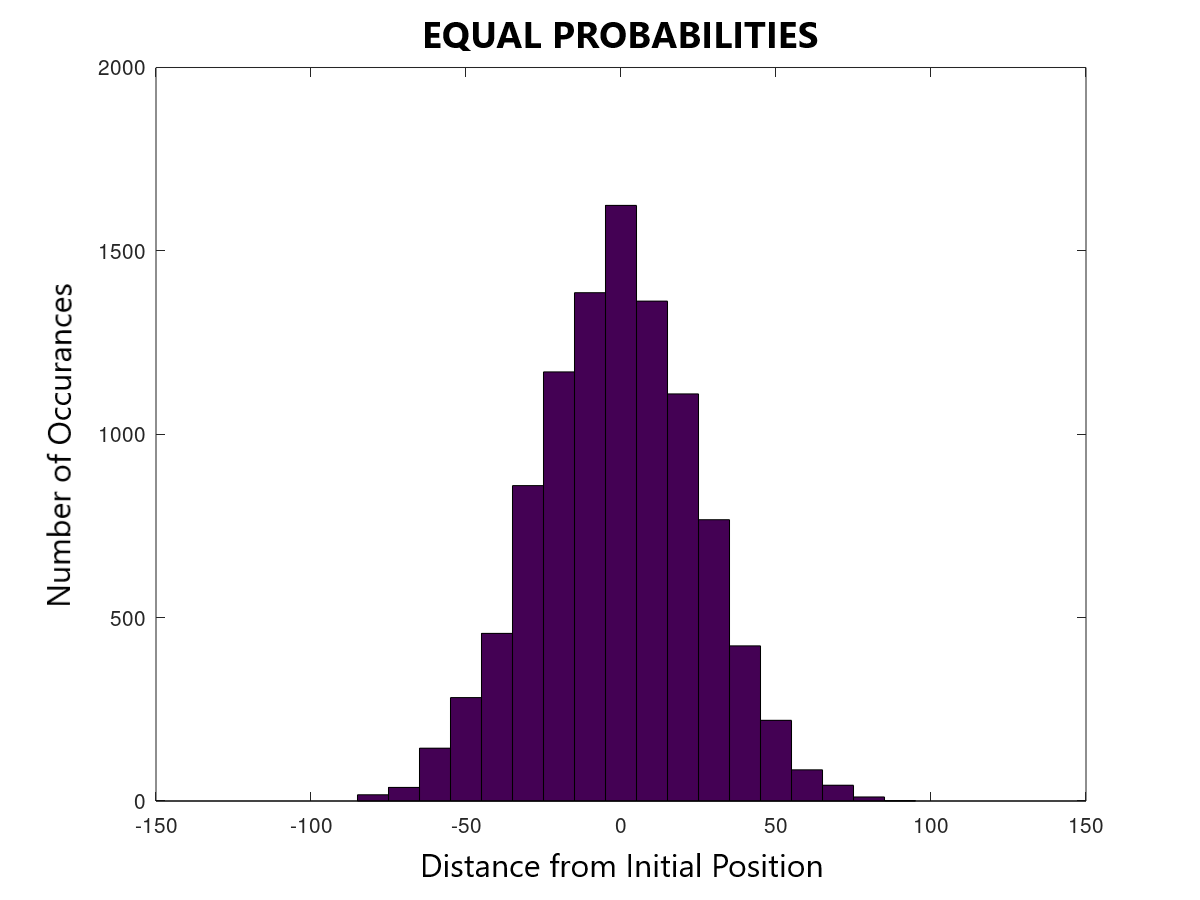
\includegraphics[width = 0.8\textwidth]{Graphs/task1_equal.png}
    \caption{Task 1 For Equal}
    \label{fig:task1_a}
\end{figure}\\
\begin{figure}[H]
    \centering
    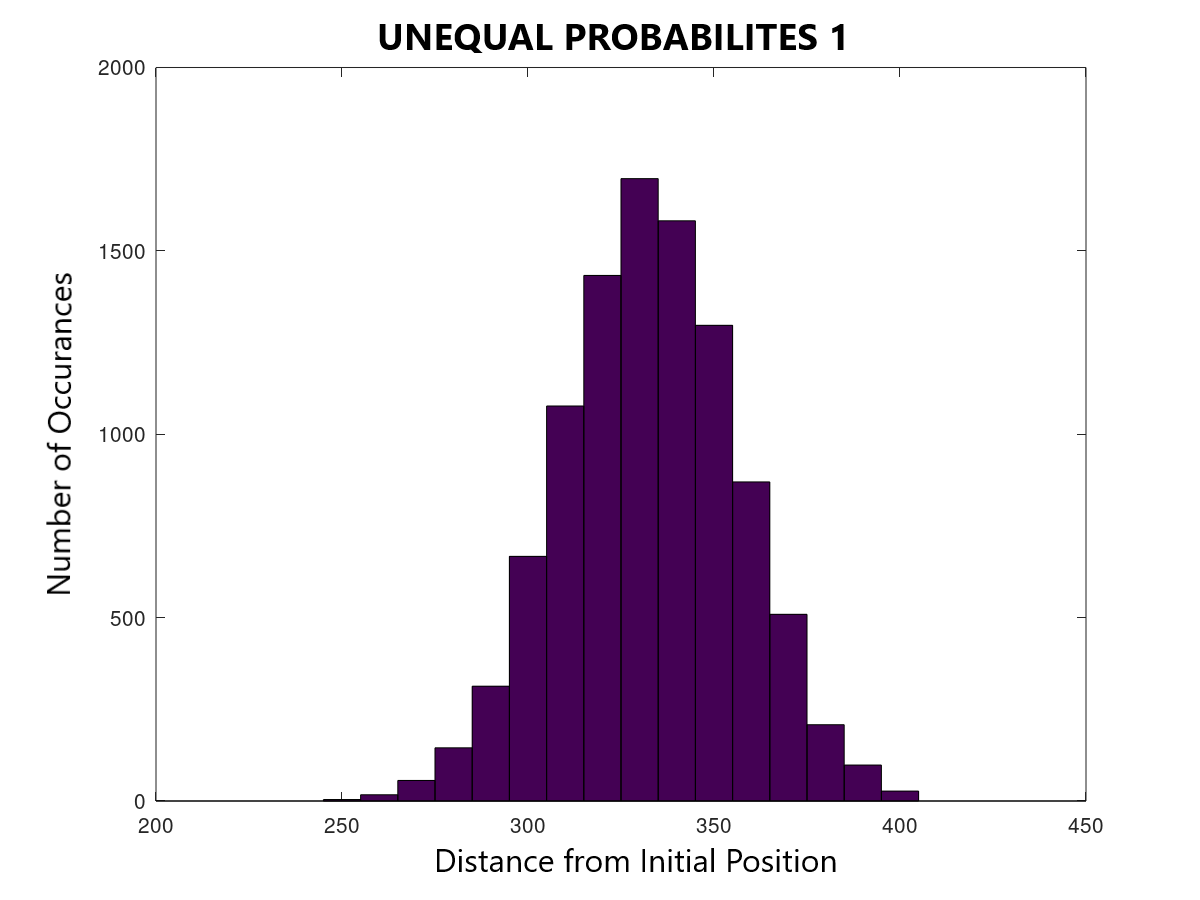
\includegraphics[width = 0.8\textwidth]{Graphs/task1_unequal.png}
    \caption{Task 1 for Unequal}
    \label{fig:task1_b}
\end{figure}\\
\subsection{Task 2}
\begin{figure}[H]
    \centering
    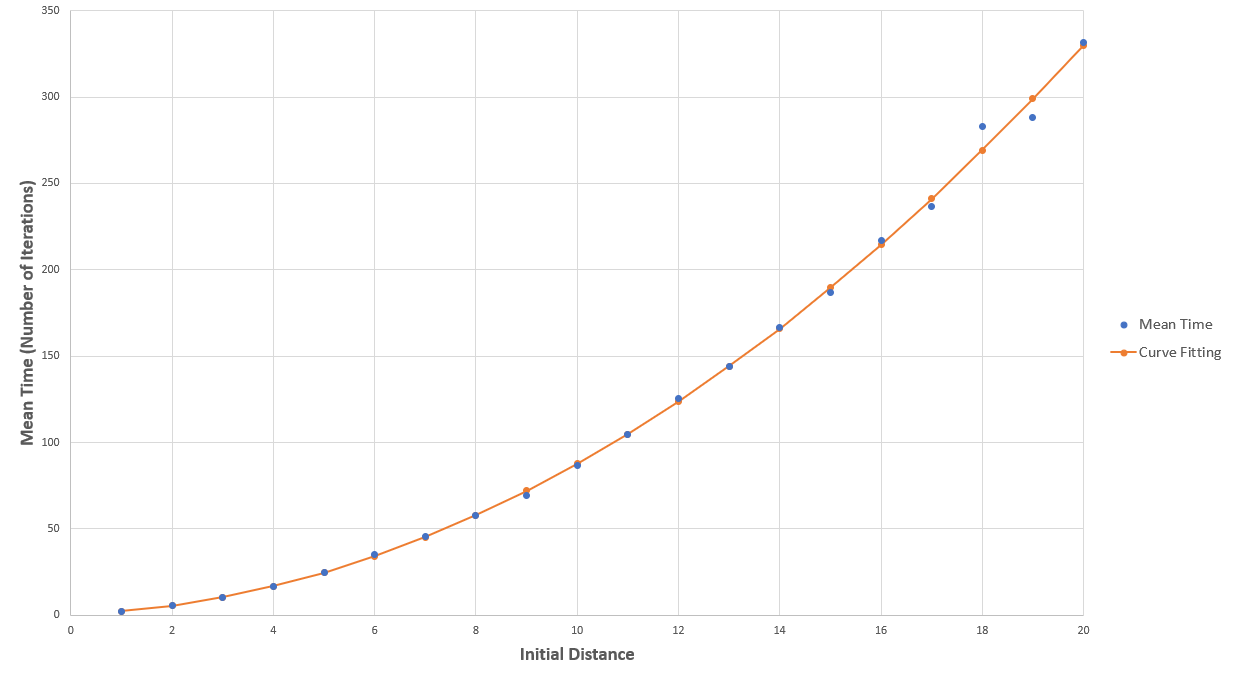
\includegraphics[width = 0.8\textwidth]{Graphs/task2.PNG}
    \caption{Task 2}
    \label{fig:task2}
\end{figure}\\
\subsection{Task 3}
\begin{figure}[H]
        \centering
        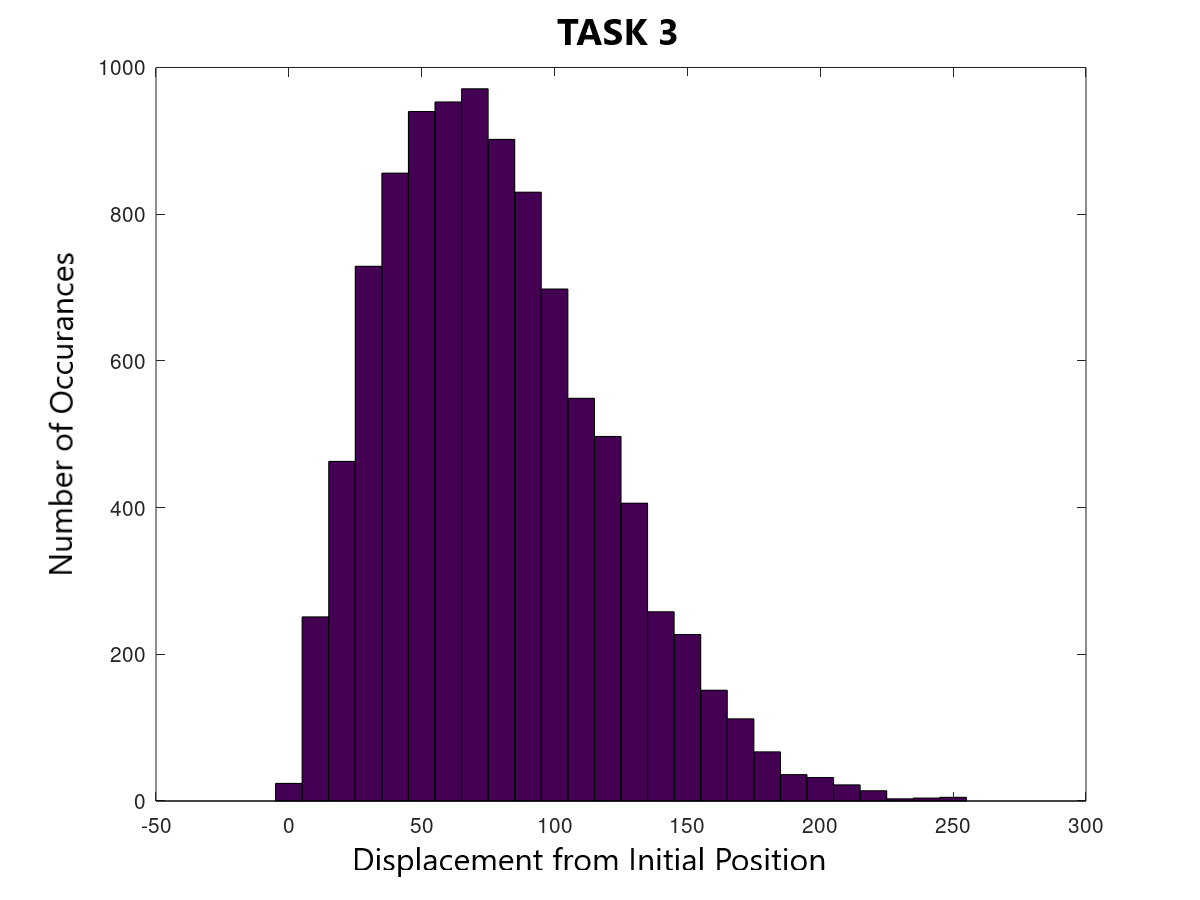
\includegraphics[width = 0.8\textwidth]{Graphs/task3.png}
        \caption{Task 3}
        \label{fig:task3}
    \end{figure}\\
    
\subsection{Task 4}
    \begin{figure}[H]
        \centering
        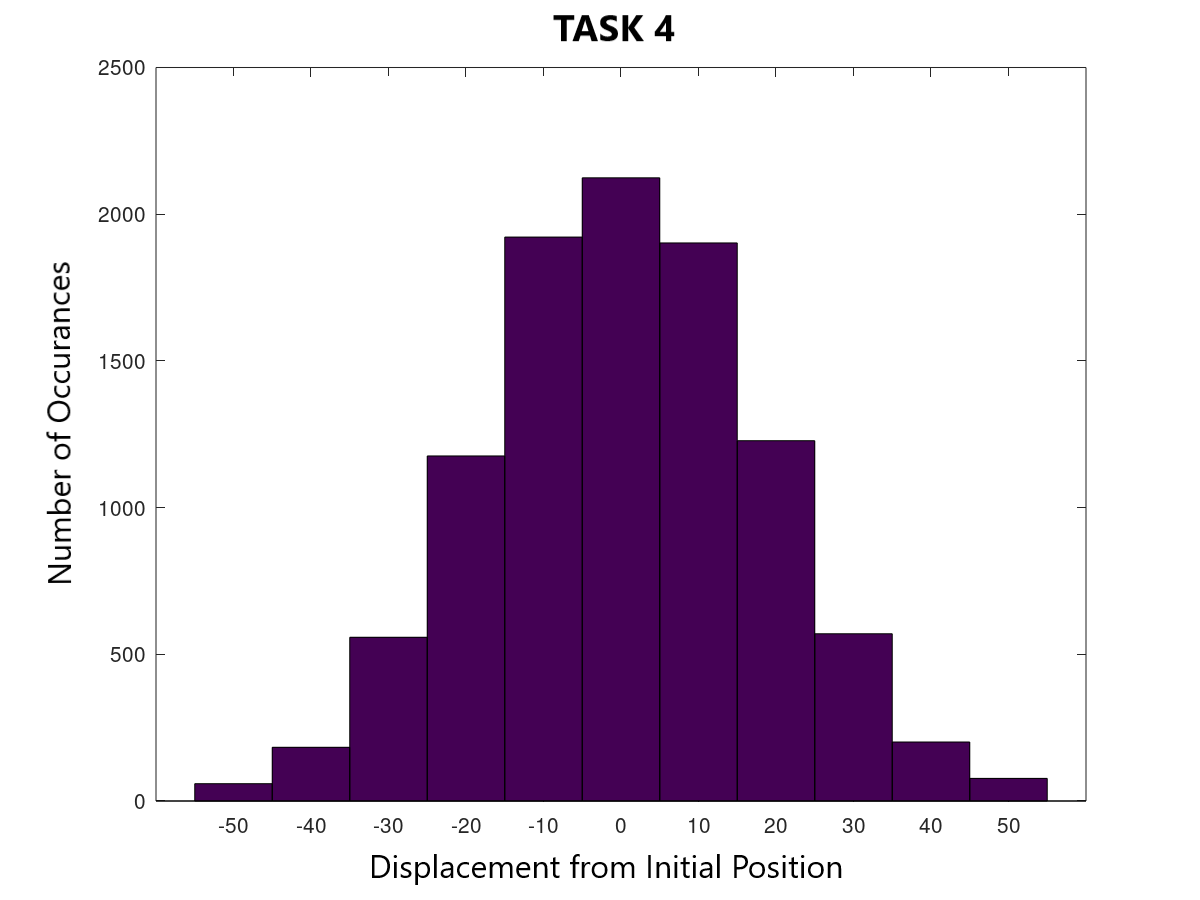
\includegraphics[width = 0.8\textwidth]{Graphs/task4.png}
        \caption{Task 4}
        \label{fig:task4}
    \end{figure}\\
    
\subsection{Task 5/6}
    \begin{figure}[H]
        \centering
        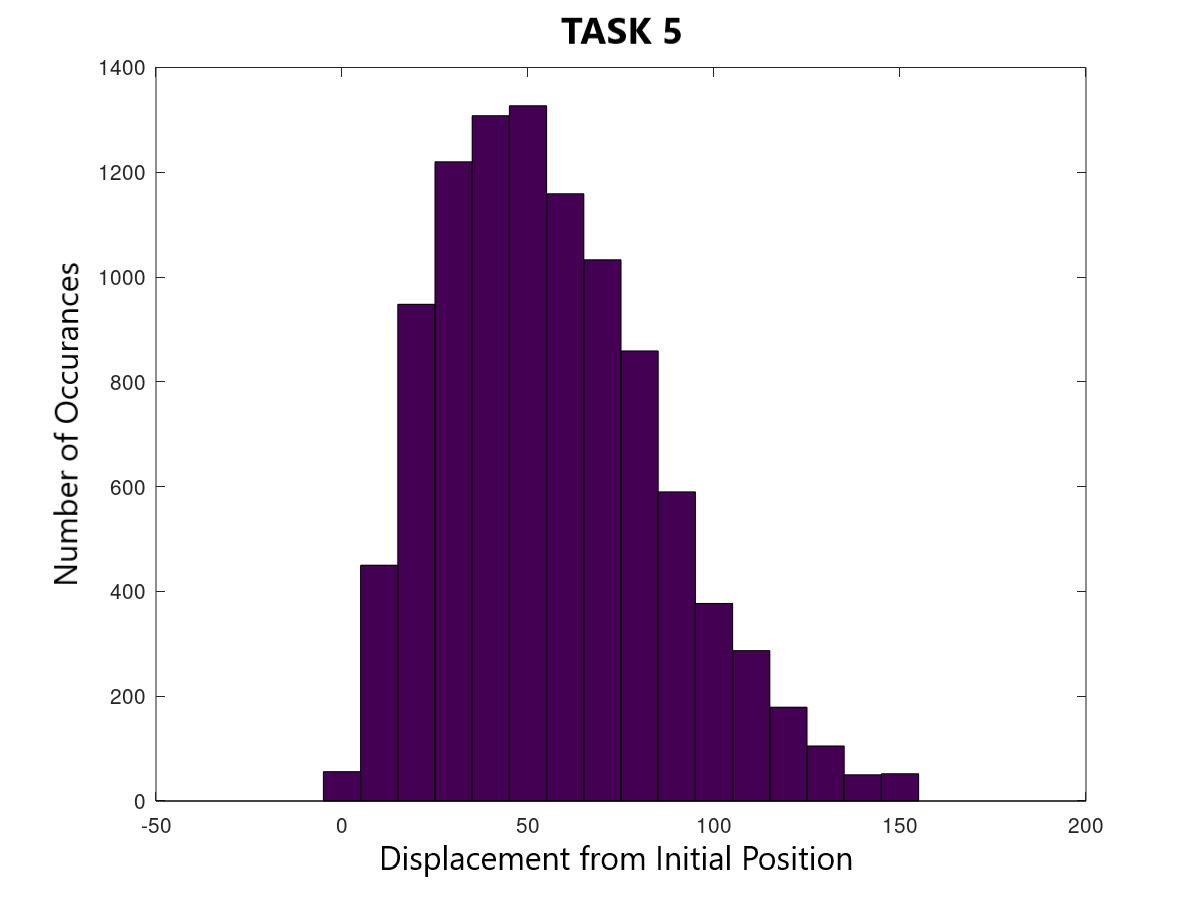
\includegraphics[width = 0.8\textwidth]{Graphs/task5.png}
        \caption{Task 5/6}
        \label{fig:task5}
    \end{figure}\\
    
\subsection{Task 7}
    \begin{figure}[H]
        \centering
        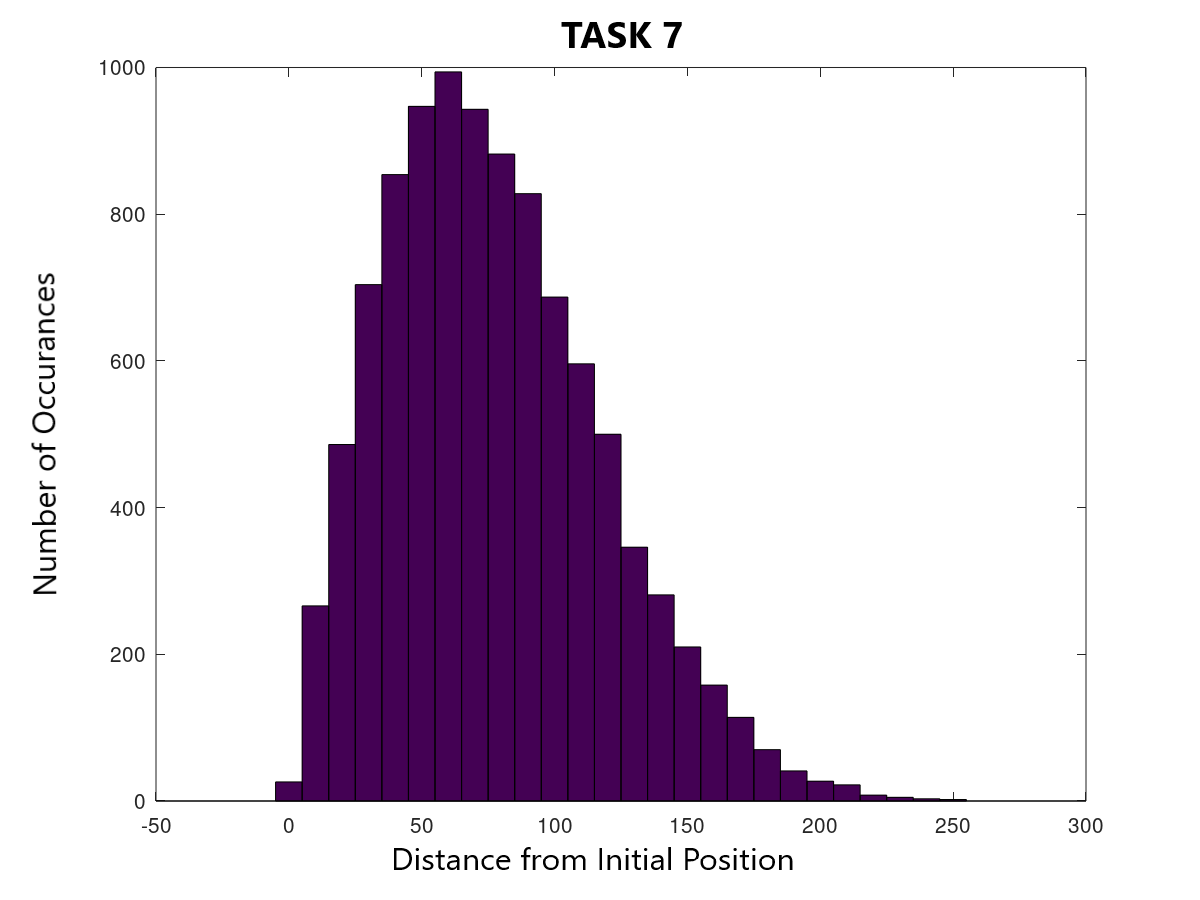
\includegraphics[width = 0.8\textwidth]{Graphs/task7.png}
        \caption{Task 7}
        \label{fig:task7}
    \end{figure}\\
    
\subsection{Task 8}
    \begin{figure}[H]
        \centering
        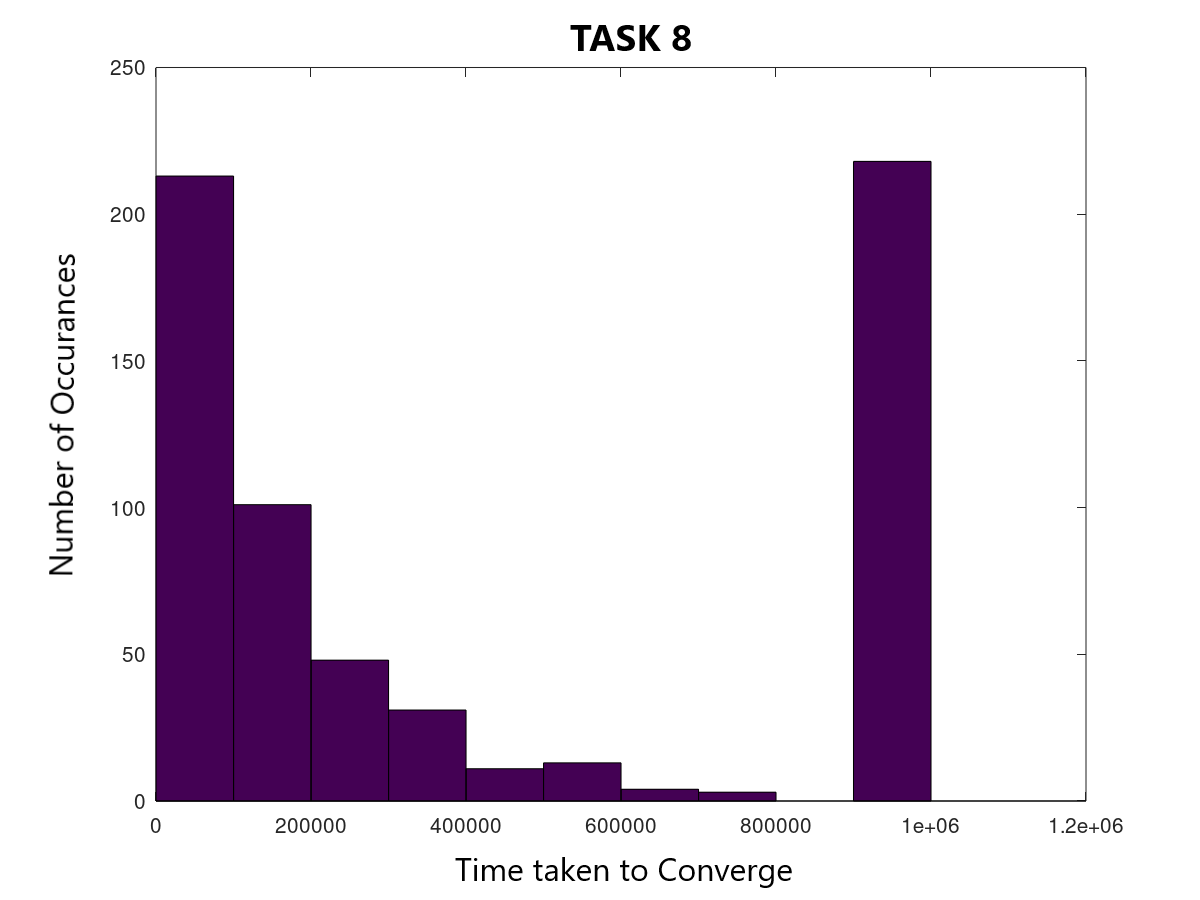
\includegraphics[width = 0.8\textwidth]{Graphs/task8.png}
        \caption{Task 8}
        \label{fig:task8}\\
    \end{figure}
    
\subsection{Task 9}
    \begin{figure}[H]
        \centering
        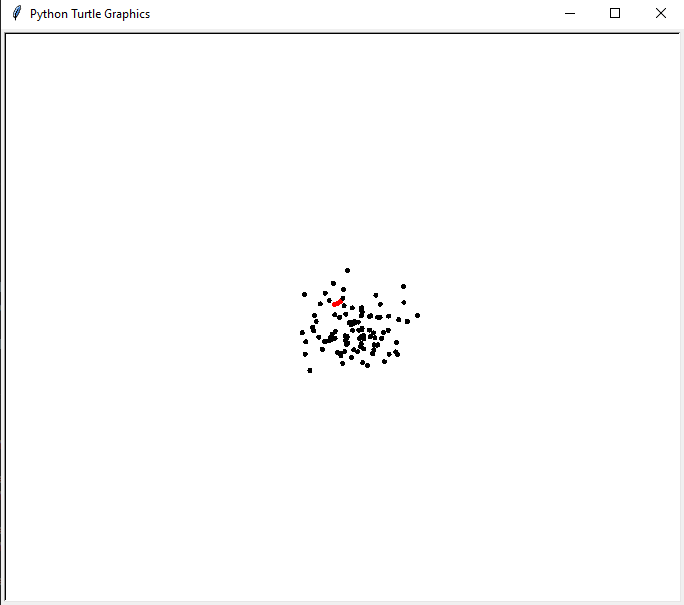
\includegraphics[width = 0.8\textwidth]{Graphs/9a.png}
        \caption{Task 9 (Close)}
        \label{fig:task9_a}
    \end{figure}\\
    \begin{figure}[H]
        \centering
        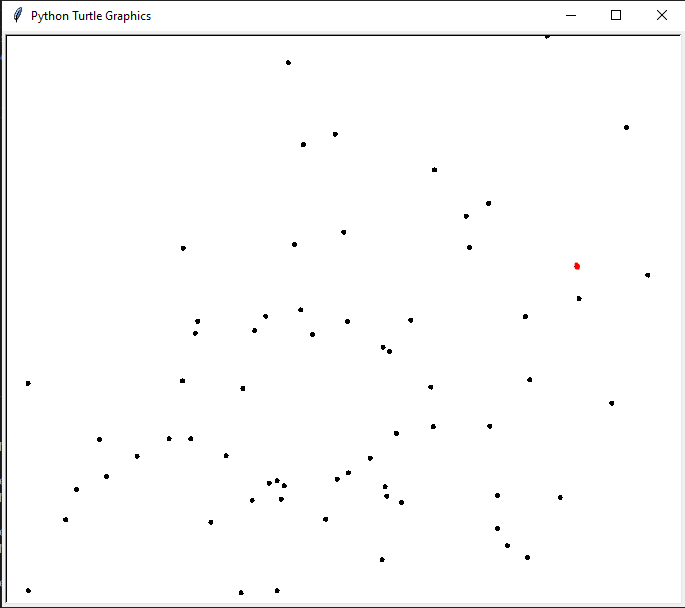
\includegraphics[width = 0.8\textwidth]{Graphs/9b.png}
        \caption{Task 9 (Scattered)}
        \label{fig:task9_b}
    \end{figure}

\section{GitHub Repository}
Please refer to our \href{https://github.com/FasihHussain22/Probability-Project/tree/master}{GitHub repository} for simulation codes

\section{References}
\begin{itemize}
    \item \href{https://www.stat.berkeley.edu/~aldous/RWG/Book_Ralph/book.html}{\text{https://www.stat.berkeley.edu/~aldous/RWG/Book_Ralph/book.html}}
    \item \href{https://blogs.sas.com/content/iml/2016/03/30/generate-uniform-2d-ball.html}{\text{https://blogs.sas.com/content/iml/2016/03/30/generate-uniform-2d-ball.html}}
\end{itemize}


\end{document}
 
